\centering
\textbf{HW Assignment \# 2 - MSE XYZ: Latex Styles} \dotfill \textbf{Fall 2024}

\rule{\textwidth}{0.4pt}
\begin{center}
\begin{tabular}{c | c | c}
     Handed Out: 8/26/24 5pm & Due: 9/2/24 5pm & Total: 25 points\\
\end{tabular}
\end{center}
\rule{\textwidth}{0.4pt}
\begin{questions}
\question[2]
The \verb|tabular| environment is useful for showing constants:
\begin{center}
    \begin{tabular}{c c c}
        $a=1$ & $N_A = \num{6.02E23}$ & $\beta=\SI{200}{\degreeCelsius\per\min}$
    \end{tabular}
\end{center}
The \verb|num{}| environment from the \verb|siunitx| package typesets scientific notation elegantly, and the \verb|SI{}{}| environment makes typesetting units quite easy.
\begin{solution}[1in]
Of course, the same thing works in the solution environment:
\begin{center}
    \begin{tabular}{c c c}
        $a=1$ & $N_A = \num{6.02E23}$ & $\beta=\SI{200}{\degreeCelsius\per\min}$
    \end{tabular}
\end{center}
\end{solution}

\question[3]
Occasionally, it might be desirable to include a plot or figure with a question.
Instead of using the \verb|figure| environment, which might not place the figure exactly where you want, I recommend using the \verb|center| environment, and the \verb|includegraphics| command, which will place the figure exactly where you want.
For example:\\
\begin{center}
    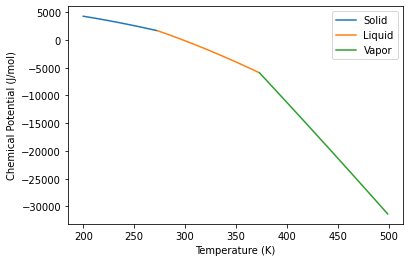
\includegraphics[width=0.5\textwidth,keepaspectratio]{figures/equilibriumplot.png}
\end{center}
After which, you can continue writing the question.

\begin{solution}[1in]
The same advice holds within the solution environment:\\
\begin{center}
    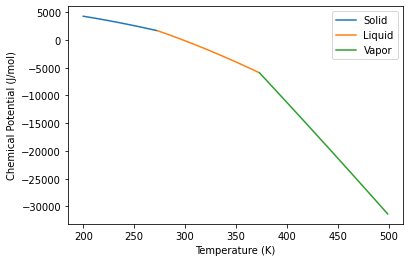
\includegraphics[width=0.5\textwidth,keepaspectratio]{figures/equilibriumplot.png}
\end{center}
\end{solution}

\question[4]
When writing math, I generally find that the \verb|align*| environment (from \verb|amsmath|) provides the best results:
\begin{align*}
    a^2 + b^2 &= c^2\\
    a^2 &= c^2 - b^2\\
    a &= \pm \sqrt{c^2 - b^2}
\end{align*}
Within the \verb|align*| environment, the \& is a special ``alignment'' character.
This allows you to line up a given equation feature (in this case, the $=$) to make things more readable.
\begin{solution}[1in]
Sometimes, it's desirable to show terms begin cancelled in solutions.
This can be accomplished using the \verb|cancel| package:
\begin{align*}
    \frac{a}{b} &= \frac{c}{b} + \frac{e}{f}\\
    \frac{a}{\bcancel{b}} \bcancel{b} &= b \left(\frac{c}{\bcancel{b}} + \frac{e}{f}\right)\\
    a &= c + \frac{b e}{f}
\end{align*}
\end{solution}

\question[5]
Sometimes it's desirable to have only a one-line equation or expression, where the \verb|align*| environment is a bit too much.
In that case, the \verb|\[\]| shorthand is quite useful, like so:
\[ q = \SI{1.602E-19}{\C\per\mol}\]
Additionally, sometimes it's necessary to tweak the sizes of parentheses or brackets in complicated expressions.
In these cases, the \verb|\left(\right)| commands are quite useful, like so:
\[ \left(\frac{\delta x}{dt}\right)_T = \left[\frac{\delta y}{dt}\right]_P \]
\end{questions}
